\section{Description of the mission}

\-\hspace{0.5cm} The launch of any roaming service is dependent on the launch of the service before it, for example we cannot launch \acs{3G} without having the \acs{2G} and \acs{GPRS} technologies already launched. same for \acs{4G} \acs{LTE} without \acs{3G}. Also, \acs{4G} \acs{LTE} must be live with a specific operator before we talk about \acs{5G} \acs{NSA} as this service on its architecture is based on the \acs{5G} radio access part and \acs{4G} core network.\\

During my internship, I have conducted the coordination in order to launch many roaming services with different operators all around the world. It gave me the opportunity to pass through all services which are going to be detailed by operator in below as the following:
\begin{enumerate}
    \setlength\itemsep{0.1em}
    \item \textbf{Airtel Sri-Lanka (41305 -LKAAT):} We have been solicited by the roaming partner to establish \acs{4G} \acs{LTE} on bilateral. Also, the launch of \acs{2G}, \acs{GPRS} and \acs{3G} services via Hub is mandatory before \acs{4G} \acs{LTE}. 
    \item \textbf{Vodafone-Cytamobile Cyprus (28001-CYPCT):} In order to launch \acs{4G} service on bilateral (\acs{RIN} and \acs{ROUT}).
    \item \textbf{Vodafone-Idea India:} in order to launch \acs{4G} \acs{LTE} on unilateral \acs{ROUT}. 
    \item \textbf{Roadmap \acs{5G} \acs{NSA} with the \acs{ROC} team:} In order to invite all the operators that we already launched \acs{4G} \acs{LTE} with, to launch \acs{5G} \acs{NSA} by default. 
\end{enumerate}

\section{The \acs{2G} service}
\-\hspace{0.5cm} The first service I started with is the \acs{2G} or \acs{GSM} which concerns only calls between mobiles. The launch of this service is necessary for the launch of any other mobile roaming service (\acs{CAMEL}, \acs{GPRS}, \acs{3G}, \acs{4G} \acs{LTE}, \acs{VOLTE}, \acs{5G} \acs{NSA}).\\

{\large \textbf{Bharti Airtel Sri-Lanka (41305 -LKAAT)}}\\

This operator solicited Orange France for \acs{4G} \acs{LTE} service establishment on a bilateral basis. However, after checking on our database and contracts archive, I found that the only services that have been launched were \acs{2G} services running on unilateral \acs{RIN} via Hub since 2016. As a result, \acs{2G}, \acs{GPRS} and \acs{3G} must be launched via hub to reach \acs{4G} \acs{LTE}.\\

\subsection{\acs{2G} architecture presentation}
\-\hspace{0.5cm} A presentation of \acs{2G} network architecture is available in annex 8 \cite{annexes}\\

\subsection{\acs{2G} Roaming Service Opening Process}
\-\hspace{0.5cm} For \acs{2G} service openings, there is a process which must be followed by the coordinators of the 2 partners operators.\\

\subsubsection{Contact operator}
\-\hspace{0.5cm} The first phase of this process consists of an initial contact with the operator. This phase is common to all service openings and contain two possible scenarios:\\

In the first case, the interest comes from Orange, through the 2022 Roadmap, the contact is initiated by the coordinator, so by me for the \acs{2G} service, and the contacted operator answers us by letting us know if they are interested or not in the proposal.\\

The second case concerns an interest initiated by operators. This interest is obviously evaluated on our side, from the geographical and tariff characteristics of the operators, as well as all the parameters taken into account for the establishment of the 2022 program.\\

If a service opening with the requesting operator is valid for us, it is added to the 2022 Roadmap.\\

During this first contact, two standard documents are always exchanged:
\begin{itemize}
    \setlength\itemsep{0.2em}
    \item The \textbf{AA14} contains the operator's privileged contacts (technical or marketing), the list of services offered in roaming, its tariff plan, and other information related to roaming.
    \item The \textbf{IR21} contains all the technical characteristics of the operator, such as its own network code (\acs{PLMN} code), billing code (\acs{TAP} code) and the key data relevant to International Roaming.
    \item In the case of services’ launch via the \textbf{HUB} as with “Bharti Airtel” Sri Lanka. Another document is provided by the roaming HUB support. IR85, this document is based on the IR21 of the roaming partner containing all the technical characteristics to launch via HUB. 
\end{itemize}

The model of these documents is written by GSMA, and they must be updated relatively often by the operators to allow good exchanges between partners.\\

\subsubsection{Contract’s negotiation}
\-\hspace{0.5cm} As soon as the two operators agree to launch services for their customers, a phase of contracts, commonly called International Roaming Agreements, starts.\\

AA.12 in conjunction with AA.13 comprises the \acs{GSM} Association standard template for international roaming agreement for parties who wish to make unilateral/bilateral agreement of international roaming services. The basic legal framework set out in AA.12 covers areas such as scope, confidentiality, provisions, data privacy, liability, fraud prevention, duration suspension of services and termination.\\

Orange France requests a certain number of "deviations" from the initial contracts, concerning in particular:

\begin{itemize}
    \setlength\itemsep{0.2em}
    \item The date of the agreement’s application and the period before suspension of the agreement in case of conflict.
    \item The periodicity of invoice exchanges.
    \item Interest rates applied in case of late payment.
    \item And other technical and financial terms …
\end{itemize}

This negotiation phase generally goes well, within a fortnight, for the most cooperative operators. However, some operators do not accept each other's specific requests and this could be the point blocking the rest of the procedures.\\

In my case with the operator “Bharti Airtel” of Sri Lanka, I did not have to negotiate the IRA with the roaming partner as it was already established in 2016 when \acs{2G} \acs{RIN} was launched.\\

\subsubsection{Tariffs' negotiations}
\-\hspace{0.5cm} In parallel with the negotiation of AA12 and AA13. A tariff negotiation phase generally starts. in particular, concerning operators presenting a financial stake.\\

The team of commercial negotiators is usually in charge of these negotiations, which often prove to be difficult and delicate to conduct.\\

The primary goal of these commercial negotiations is to reduce customer charges, calculated in the form of an average tariff, called \acs{IoT}. This tariff is calculated on a yearly basis.\\

\textbf{Inter-Operator Tariff} means the wholesale rates charged between two roaming partners. The \acs{IoT}s shall be calculated as the outbound roaming traffic weighted average per country. This entails calculating a weighted average of the \acs{IoT}s faced by each \acs{MNO} within a specific country.\\

The commercial negotiators have different means to push on the roaming partners in order to close the best deal for Orange France customers, as the following:\par
\begin{itemize}
    \setlength\itemsep{0.2em}
    \item Launch services with several competing operators in the same country, that is going to create competition between them.
    \item Traffic redirection or what we call Steering, which allows us to distribute Orange France customers roaming internationally to the different partner networks in the country. The steering tool directs the maximum traffic to the operator offering us the best price.
\end{itemize}

With the operator “Bharti Airtel” of Sri Lanka, we did not have a deal before for our customers, so I had to communicate with the commercial negotiator responsible for that operator’s region in order to get the best deal. He gave me the green light to start the phase of testing.\\

\subsubsection{Tests Coordination}
\-\hspace{0.5cm} After this commercial phase, comes another phase of my mission, which is the management of technical tests and invoicing, also the coordination of all the actors involved.\\

First, I initiate the technical tests by an implementation request of the \acs{SIM} cards of the operator in which we want to open the \acs{2G} service with, the implementation takes a period of 3 weeks, in this request, I specify the type of launch (bilateral or unilateral) and I provide the technical team with the \acs{SIM} cards details and IR21 of the operator, or IR85 in case of launch via hub. \\

Also, I ensure the good exchange of \acs{SIM} cards in the shortest possible time (I will get into this part within the coming sections), and the Testbooks between the roaming partners’ technical teams who are called “IREG”. \\

A testbook is a standard book proposed by the \acs{GSMA} that contains a process of tests regarding localization, calls and \acs{SMS} tests … etc.\\

As soon as the implementation is effective, on our \acs{MSC} for an opening in Roaming IN or on our \acs{HLR} and \acs{MSC} for an opening in Roaming OUT, I warn our \acs{DCH} , MACH, that tests are going to start, and I provide them with the tariffs of the roaming partner via a system called “service ticket” via their website.\\

Once the tests finish, the testbook is going to be sent with the \acs{TAP} files to the roaming partner’s \acs{IREG} team. If this last is validated by the IREG, a technical GO is issued, which is the starting point for the billing tests conducted by the \acs{TADIG} team (Transferred Account Data Internet Group).\\

These tests consist of a verification of the correct valuation of our customers’ calls "roaming" abroad, by our platforms (called \acs{ADV} for our mass market customers and \acs{DISE} for our business market customers).\\

The testing phase is completed by issuing a test completion certificate \acs{TCC}, by both operators. This phase is obviously the longest. In the best case, it can take a fortnight for all the steps. However, most of the tests face technical difficulties, with some operators, it takes months to be completed.\\

For the operator Bharti Airtel, we do all the steps with the roaming HUB as it is our interface to launch with the operator. The tests phase did not start yet with the Sri-Lankan operator because I started working with them at the end of august.\\

\subsubsection{Commerciale launch}
\-\hspace{0.5cm} After the validation of all the tests, my mission is to negotiate with the operator the effective date and the modalities (unilateral or bilateral) of \acs{2G} commercial launch.\\

Once the date is fixed, a \acs{CLL} (Commerciale Launch Letter) is signed by both parties. I conclude the procedure with a launch announcement via email to:
\begin{itemize}
    \setlength\itemsep{0.2em}
    \item Technical team in order to do network generalization.
    \item Our assistant in order to update the database.
    \item To all the department’s team.
\end{itemize}

Orange France provides all its customers with an interface, called “Pass voyage”, via the official website, on which the new services and destinations launched during the month are updated.\\

\section{\acs{GPRS} and \acs{3G} service}
\-\hspace{0.5cm} General packet radio service (\acs{GPRS}) Also called DATA, is essentially a packet-switching technology that allows information to be transmitted via mobile networks. It is utilized mostly for internet connectivity.\\

In the roaming world, \acs{GPRS} service allows orange France customers to use data browsing under other operators’ networks. The \acs{3G} is based on the composition of voice \acs{2G} and DATA \acs{GPRS}. So, in order to launch \acs{3G} service, \acs{2G} and \acs{GPRS} must be already launched. \\

\subsection{\acs{GPRS} and \acs{3G} architecture presentation}
A presentation of \acs{GPRS} and \acs{3G} network architecture is available in annex 8 \cite{annexes}

\subsection{\acs{GPRS} and \acs{3G} Roaming Services opening Process}
\-\hspace{0.5cm} The procedure of \acs{GPRS} roaming service opening is related to the \acs{2G} procedure, we already have the \acs{SIM} cards of the operator as well as the IR85 as we launch via HUB. Also, we don’t have to do contracts and commercial negotiations because it was already done at the first contact for \acs{2G} opening. For \acs{3G} service, Orange France prefers launch by default without \acs{IREG} testing and \acs{TADIG} validation because the \acs{3G} architecture is directly based on the architecture of \acs{2G} and \acs{GPRS}.\\

In order to simplify the internship report, I have chosen to pass directly to the testing phase.\\

\subsubsection{Tests Coordination}
\-\hspace{0.5cm} The testing phase of \acs{GPRS} is similar to the \acs{2G} service testing. However, as data services are more complicated to implement, a questionnaire \acs{GPRS} needs to be filled by the roaming partner in order to have answers and clear vision of their architecture. This questionnaire contains \acs{IREG} and \acs{TADIG} requirements to pass successful tests. \\

Once I have the IR85, the data of the \acs{SIM} cards and the questionnaire filled by the roaming partner, I do the \acs{GPRS} implementation request via email which takes 3 weeks to be done. During this period, I make sure to send our \acs{GPRS} testbook IR35 to the roaming partner and receive their IR35 as the opening is going to be in Bilateral (\acs{RIN} \& \acs{ROUT}).\\

The tests start as the implementation takes place, because the launch is on a bilateral basis, the \acs{IREG} team of the roaming partner uses our \acs{SIM} cards to perform tests under their network and fill our testbook. Also, our \acs{IREG} team uses the Partner’s \acs{SIM} cards to perform tests under Orange France network and fill their testbook. As a part of my tasks, I ensure the communication between the two \acs{IREG} teams. Sometimes I do plan a meeting through Teams or Skype in order to solve the testing problems as soon as possible.\\
	
As long as the tests finish, the \acs{IREG} partners exchange the completed testbooks with the \acs{TAP} file. If the tests and the \acs{TAP} files are validated, the technical teams sign the test completion certificate \acs{TCC}.\\

Like I have mentioned before, \acs{3G} service opening does not need any tests completion or \acs{TADIG} validation because it was already done with \acs{2G} and \acs{GPRS}.\\

\subsubsection{Commerciale launch}
\-\hspace{0.5cm} My role in this part is similar to the \acs{2G} procedure, I negotiate with the coordinator of the roaming partner to agree on an official commercial launch date. Once we agree on a date, I make a request for a network generalization via an email to the technical team, and I proceed with the \acs{CLL} signature. Legally As an intern, I don’t have the authority to sign such a document, so I pass the launch letter to my manager to countersign with the Roaming partner and then save this document in our archives and do the launch announcement.\\

For \acs{3G} launch by default, a request of implementation and generalization is done via the same email, I highlight a launch date and countersign the \acs{CLL} with the roaming partner directly.\\

I am going to mention the \acs{4G} roaming service in the next titles with different opérators.\\

\section{\acs{4G} \acs{LTE} service}
\-\hspace{0.5cm} \acs{4G} \acs{LTE} is short for “fourth generation long-term evolution”. So, it’s actually two terms combined. First, “\acs{4G}” represents the fourth generation of mobile technology, the next big advancement after \acs{3G}. And “long-term evolution,” or “LTE,” is industry jargon used to describe the particular type of \acs{4G} that delivers the fastest mobile internet experience. \cite{4glte}\\

\subsection{\acs{4G} architecture presentation}
\-\hspace{0.5cm} A presentation of \acs{4G} network architecture is available in annex 8 \cite{annexes}\\

\begin{itemize}
    \item {\large \textbf{Vodafone-Cytamobile Cyprus (28001-CYPCT)}}\\
\end{itemize}

With this operator, I have been asked by my manager to contact the operator Vodafone-Cytamobile in Cyprus in order to open the service \acs{4G} on a bilateral basis.\\

I have checked on our database \acs{OliveRA} to see what action should be taken regarding the other services that must be launched before \acs{4G} LTE.  \\

Based on \acs{OliveRA}, \acs{3G} has already been launched on a bilateral basis since 2006. So, I can proceed directly with \acs{4G} service.\\

\subsection{\acs{4G} Roaming Service Opening Process}

\subsubsection{Tests Coordination}
\-\hspace{0.5cm} The Testing procedure is always similar to the standard one of \acs{2G} service. However, with this operator Vodafone-Cytamobile as we launched all the other services a long time ago, I had to go through a \acs{SIM} audit because we have sent testing \acs{SIM} cards a long time ago to the operator.\\

The \acs{SIM} audit procedure is to make sure that our \acs{IREG} team still has the \acs{SIM} cards of the roaming partner. On the other side, the roaming partner’s \acs{IREG} team has Orange France \acs{SIM} cards. Also, if the size of the \acs{SIM} cards is compatible with nowadays phone mobiles in order to perform testing.
On our side, I wrote an email to our \acs{IREG} team that contains the data of the \acs{SIM} cards asking if they still have it in possession. Our team confirmed the possession of the operator’s cards.\\

I did conclude that the Orange France \acs{SIM} cards that were sent before to the operator were old and are not nano Cards. In this situation I had to order new cards from our assistant responsible for the \acs{SIM} cards management. For \acs{4G} service, the roaming partner needs 4 \acs{SIM} cards for testing, Two \acs{ADV} (mass market customers) and two \acs{DISE} (Business market customers).\\

Also, I had to confirm the delivery address with the roaming partner to deliver the Cards. The delivery takes a few days to reach, depending on the destination. Sometimes we get some issues with the customs and our cards never reach their destination.\\

Once the roaming partner receives our cards, the coordinator confirms the reception with a picture of the cards asking for its details. The details of the cards are not sent with the package for reasons of security and fraud prevention.\\

For \acs{LTE} service, we also have a testbook called IR38, and a \acs{4G} questionnaire must be filled by the roaming partner. After a few weeks of exchanging with the other part coordinator, the \acs{SIM} cards and the testbooks were exchanged, the questionnaire was filled, and the implementation request was done. Now, both parties are ready for tests.\\

The tests were completed as well as the testbooks after 2 weeks and the \acs{TAP} files shared for validation. Also, the \acs{TCC} was signed by both parties.
I have shared the first page of the Orange France testbook completed by the roaming partner in annex 9.\\

\subsubsection{Commercial launch}
\-\hspace{0.5cm} After \acs{TCC} is signed, we are now ready for generalization, \acs{CLL} countersign and launch announcement. However, the operator Vodafone-Cytamobile requested renegotiation of the IRA signed in 1995 as it does not support the provision of \acs{LTE} and \acs{5G}.\\

\begin{itemize}
    \item {\large \textbf{Vodafone-Idea India}}\\
\end{itemize}

This is the most complicated project I worked on during my internship. India is divided up into 22 telecom circles, with multiple operators licensed to operate in each. so, we must open \acs{4G} service with 22 networks instead of one as we do with operators in different countries. Also, the name of the operator Vodafone-Idea (VI) came from the merge of the two operators Vodafone Group and Idea Cellular. This project started years ago and the operator VI didn’t have enough resources to perform tests for our customers, as a result only Rin was launched (VI customers under Orange France network) in the past years.\\

\subsection{\acs{4G} Roaming Service Opening Process (Different testing process):}
\-\hspace{0.5cm} My first action within this project was to make a list of all the existing networks under these two operators, investigate which of the networks were kept after the merge and which of them were closed in order to know the networks I need to open \acs{4G} with.\\

Based on our database and last year's previous emails exchange, I prepared a list of all networks, and I organized a meeting through Teams with the coordinator of VI to further exchange about their technical merger strategy and clarify the operations required to ensure a good user experience under merged Vodafone Idea networks.\\

After the meeting, I concluded that the total networks are 29, Idea had 22 networks and Vodafone 7. Only 21 were kept after the merge, some of them are used only for outbound roaming (\acs{ROUT}) and the rest for inbound (Rin). based on my investigation and the meeting’s information I came up with the following table which contain the networks that we need to open \acs{4G} service with:

\begin{table}[h!]
    \begin{tabular}{c}
        \raisebox{-\totalheight}{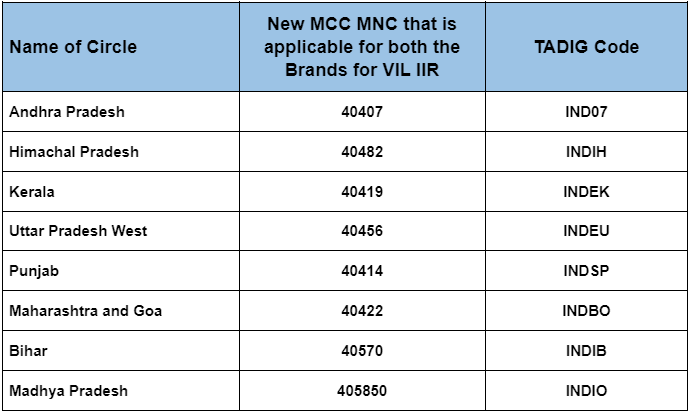
\includegraphics[scale=0.8]{part3/india.png}}
\end{tabular}
\caption{List of VI networks that should be launched}
\end{table}

\subsubsection{Tests Coordination}
\-\hspace{0.5cm} During the meeting with VI roaming coordinator, they proposed to launch \acs{4G} by default for our customers under VI networks without any \acs{IREG} testing and \acs{TADIG} validation. However, Orange France does not accept to launch by default the \acs{4G} service, especially in such a complicated situation of many networks with such an operator.\\

In this situation, I organized a meeting with my manager and my team to discuss the testing procedure with VI and we have agreed to do remote tests via SIGOS if this later covers all the telecom circles that we are interested in. \\

SIGOS allows Orange France’s \acs{IREG} team to perform tests via a remote tool and complete our IR38 without sending physical \acs{SIM} cards (With VI, there can be more than 20 cards distributed in the 8 areas). The only thing needed from the \acs{IREG} team of the roaming partner is to implement the data of our \acs{SIM} cards under their networks as the \acs{4G} service is on \acs{ROUT} basis.\\

As SIGOS covers all the networks of the telecom circles that are yet to be launched, my task now is to prepare the data of the \acs{SIM} cards and convince VI team to implement it under their networks as they wanted to launch \acs{LTE} for our customers by default. See Annex 10 about the \acs{SIM} cards’ data that I presented in my email to VI.\\

After many email exchanges with the roaming partner team, they agreed to implement our card’s data in June. However, after many emails’ reminder still the implementation is not yet done as the roaming partner is not active to our request.\\

Whenever the implementation is done, our \acs{IREG} team will perform the tests, complete the IR38 and perform the necessary checking and \acs{TADIG} validation to get the \acs{TCC} signed. \\

\subsubsection{Commerciale launch}
\-\hspace{0.5cm} After we will get the \acs{TCC} signed, the official commercial launch is similar to the previous parts, the only difference is the various networks. But still, we need to countersign only one \acs{CLL} with all the networks mentioned on.\\

\section{\acs{5G} \acs{NSA} service}
\-\hspace{0.5cm} In this part of the report, I am not going to talk in detail about the process of launch as it is similar to the previous ones. Instead, I’m going to talk about numbers, our objective, the roaming center, our process with the \acs{ROC} and expectations.\\

\subsection{The Objective}
\-\hspace{0.5cm} \acs{5G} \acs{NSA} is a new technology started in 2021, all the French operators started the race to launch this service with the maximum number of operators in order to expand their \acs{5G} \acs{NSA} coverage map to provide the best experience for their customers. \\

Orange France set up a roadmap to launch \acs{5G} \acs{NSA} with more than 80 operators by the end of 2022. As a result, our management Hired the \acs{ROC} team from Abidjan (Ivory coast) in March to accelerate the service opening.\\

\subsection{The roaming center Abidjan}
\-\hspace{0.5cm} Under the responsibility of Orange \acs{WLoB} (wholesale line of business) in Ivory coast. The Roaming Center (\acs{ROC}) is a center of expertise for roaming connectivity management that carries out and supervises roaming service openings and supports daily business activities of affiliates.

\subsection{\acs{5G} \acs{NSA} architecture presentation}
\-\hspace{0.5cm} A presentation of \acs{5G} \acs{NSA} network architecture is available in annex 8 \cite{annexes}

\subsubsection{\acs{5G} \acs{NSA} Roaming Service Opening Process}
\-\hspace{0.5cm} My role within this project is to lead the \acs{ROC} team on the process of \acs{5G} \acs{NSA} service opening. As the architecture of this technology is based on a new \acs{5G} radio access part and \acs{4G} core network, Orange France prefers to launch \acs{5G} \acs{NSA} by default without any \acs{IREG} testing and \acs{TADIG} validation with all operators to accelerate the process of opening. \\

With the Roaming center team, we have set up a plan in order to contact all the operators that we are already \acs{4G} live with. I had to Prepare a list of 40 up to 50 operators to be contacted by the \acs{ROC} each week, the lists depend on our marketing and commercial priorities.  \\

I organize each Friday a meeting via Teams with the \acs{ROC} in order to get updates about the operators accepted to launch with us, the process and dates of launch. \\

Till the end of September, we have got the following numbers resumed in the below table:

\begin{table}[h!]
    \begin{tabular}{c}
        \raisebox{-\totalheight}{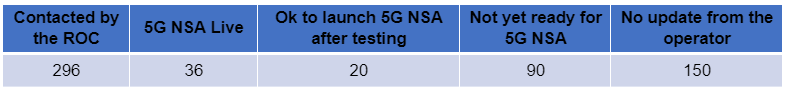
\includegraphics[scale=0.7]{part3/roc.png}}
    \end{tabular}
    \caption{Operators contacted by the ROC}
\end{table}

We have contacted 296 operators, 36 of them accepted our \acs{5G} \acs{NSA} invitation and we already launched with them. Also, 20 operators accepted to launch but after testing which is going to take more time. 90 operators are not yet ready for \acs{5G} \acs{NSA} and 150 did not give any feedback.

\begin{figure}[H]
    \centering
    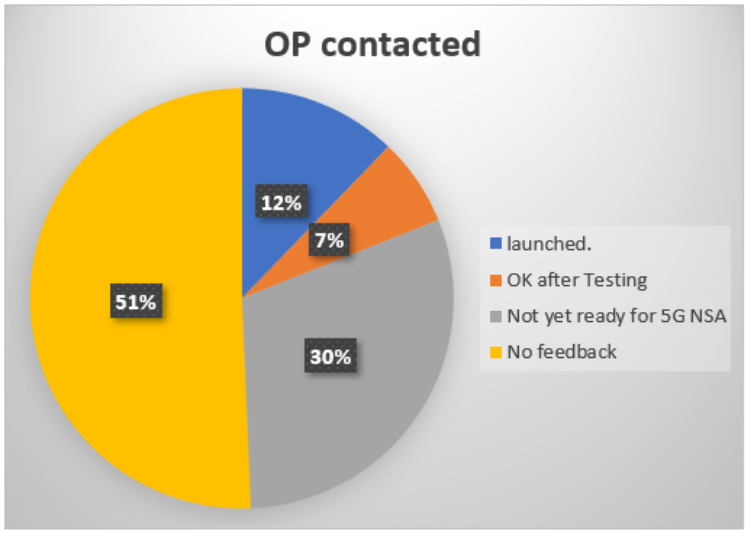
\includegraphics[scale=0.4]{part3/opcontacted.png}
\caption{Percentage of contacted operators}
\end{figure}

Also, the coordinators of The \acs{DRI}  take in charge some operators for \acs{5G} \acs{NSA} launch. In total between the \acs{DRI}  and the \acs{ROC}, we reached 86,25\% of our objective with 69 operators where 46 operators in which \acs{AAZOR} included. This number gives Orange France presence in 36 countries distributed as in the following map:

\begin{table}[h!]
    \begin{tabular}{c}
        \raisebox{-\totalheight}{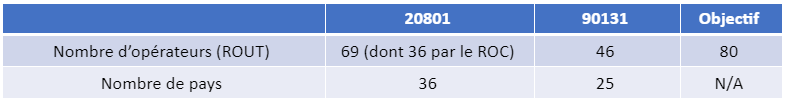
\includegraphics[scale=0.7]{part3/dri.png}}
\end{tabular}
\caption{Orange Footprint}
\end{table}

\begin{figure}[H]
    \centering
    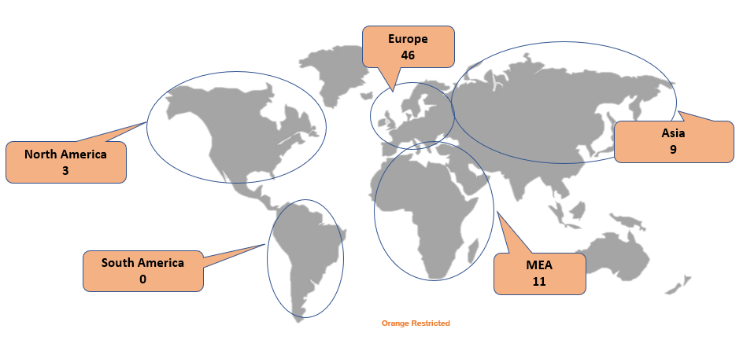
\includegraphics[scale=0.7]{part3/world.png}
\caption{Orange France 5G NSA Coverage Map}
\end{figure}

We have 46 launches in Europe as the European operators are more active, were ready for \acs{5G} \acs{NSA} and shared the same interests with us. 11 openings in MEA including 2 operators of Qatar (Vodafone \& Ooredoo) which are a higher priority for Orange France as the football world cup is starting soon. \\

I took charge of the launch with Ooredoo Qatar instead of the \acs{ROC} as the situation was delicate, we invited this Operator for \acs{5G} \acs{NSA} months ago and we had no feedback from them. After sending many kind reminders to the coordinators, I have chosen to call by phone. The person in charge answered my call and agreed to launch \acs{5G} \acs{NSA} with Orange France. We both agreed on 29th of august as a launch date. I prepared the \acs{CLL} for a bilateral launch, got it signed by my manager and sent it to the coordinator for a countersign. \acs{CLL} shown in annex 11. \\

During my internship, the most difficulties we faced are the non-active operators where it takes months to launch with them as it takes a while to get their feedback after many relance. Also, the sick leave of the roaming center person in charge. The standard process of launching \acs{5G} \acs{NSA} also takes months as the \acs{SIM} cards exchange and tests take a long time.\\

\subsection{Prospect solutions and expectation}
\-\hspace{0.5cm} I have proposed some of the solutions to my manager and to our department’s director in order to accelerate \acs{5G} \acs{NSA} launch with operators. The solutions are the following:
\begin{itemize}
    \item Insist on the operators that require testing to launch on a unilateral basis for Orange France customers before testing, and for their customers after testing. 
    \item Elaborate new \acs{5G} \acs{NSA} testbook (Light testbook) in order to make the tests simple for the operators that require tests before launch as we prefer default launch. 
    \item Prepare a list that contains 50 operators (from the 150 operators given no feedback) with higher marketing and business priority in order to contact them directly by phone instead of relancing through emails.  
    
\end{itemize}

By the end of 2022, I expect that Orange France will be able to launch with more than 110 operators. 20 operators already accepted the launch, waiting for the testing phase to complete before 2023. From the 90 operators not yet ready for \acs{5G} \acs{NSA}, I expect at least 10 of them will be ready in the last quarter of the year. Also 15 operators from the list of 50 to be contacted by phone will accept to launch with Orange France. The total could be 114 operators within 69 already launched. 




